\chapter[Proposal for an improved design]{Proposal for an improved design}\label{chap:new_design}

Chapter~\ref{chapter:CLEAR_test} showed that the ChDR emission can be used to detect the beam position of a relativistic charged-particle beam. In this chapter, the experience gained with the test device at CLEAR is extrapolated to the possible application of this technique at AWAKE by using electromagnetic simulations and scaling laws. 


\section[Coupling to the proton beam]{Coupling to the proton beam}

The main difference between the test conditions at CLEAR and in the AWAKE beamline is the presence of the proton beam. Chapter~\ref{chapter:copropagating_beams} showed that carrying out the measurement at high-enough frequency is sufficient to detect the electron beam with reduced contribution from the protons. Using a design similar to the one tested at CLEAR exploits the inherent insensitivity of ChDR to low-frequency signals.

According to the PCA theory, electromagnetic radiation is produced on the surface of a dielectric radiator and then propagates through it. In the geometry examined in this work, the radiator is cylindrical and surrounded by metal. Therefore, the electromagnetic wave propagates de facto through a circular waveguide filled with the radiator dielectric material. The cutoff frequency of the fundamental mode of a dielectric-loaded circular waveguide is
\begin{equation}
f_c=\frac{1.8412c}{2\pi r} \frac{1}{\sqrt{\epsilon_r}} \label{eq:cutoff_loaded}
\end{equation}
where $r$ is the waveguide radius, $c$ the speed of light in vacuum and $\epsilon_r$ the relative permittivity of the dielectric material~\cite{Jackson:490457}. 

The prototype device tested at CLEAR featured PTFE radiators with a radius of 9~mm, resulting in a cutoff frequency of 6.74~GHz. Using the 3D model presented in Section~\ref{sec:single_electrode}, it is possible to simulate the response of the device to bunches of varying length and charge. Figure~\ref{fig:protons_in_clear} shows the electric-field magnitude computed at the location indicated in Fig.~\ref{fig:sim_t_scan}~(a) when simulating proton and electron beams with parameters as in Table~\ref{tab:sim_param_comparison}. It can be immediately noted that, even though the proton-beam electric field decreases at frequencies above 0.1~GHz, it is still higher than the electron beam field up to $\sim$1~GHz (see Fig.~\ref{spectrum_run2} for a comparison of the beam spectra).




\begin{figure}[!b]
\centering
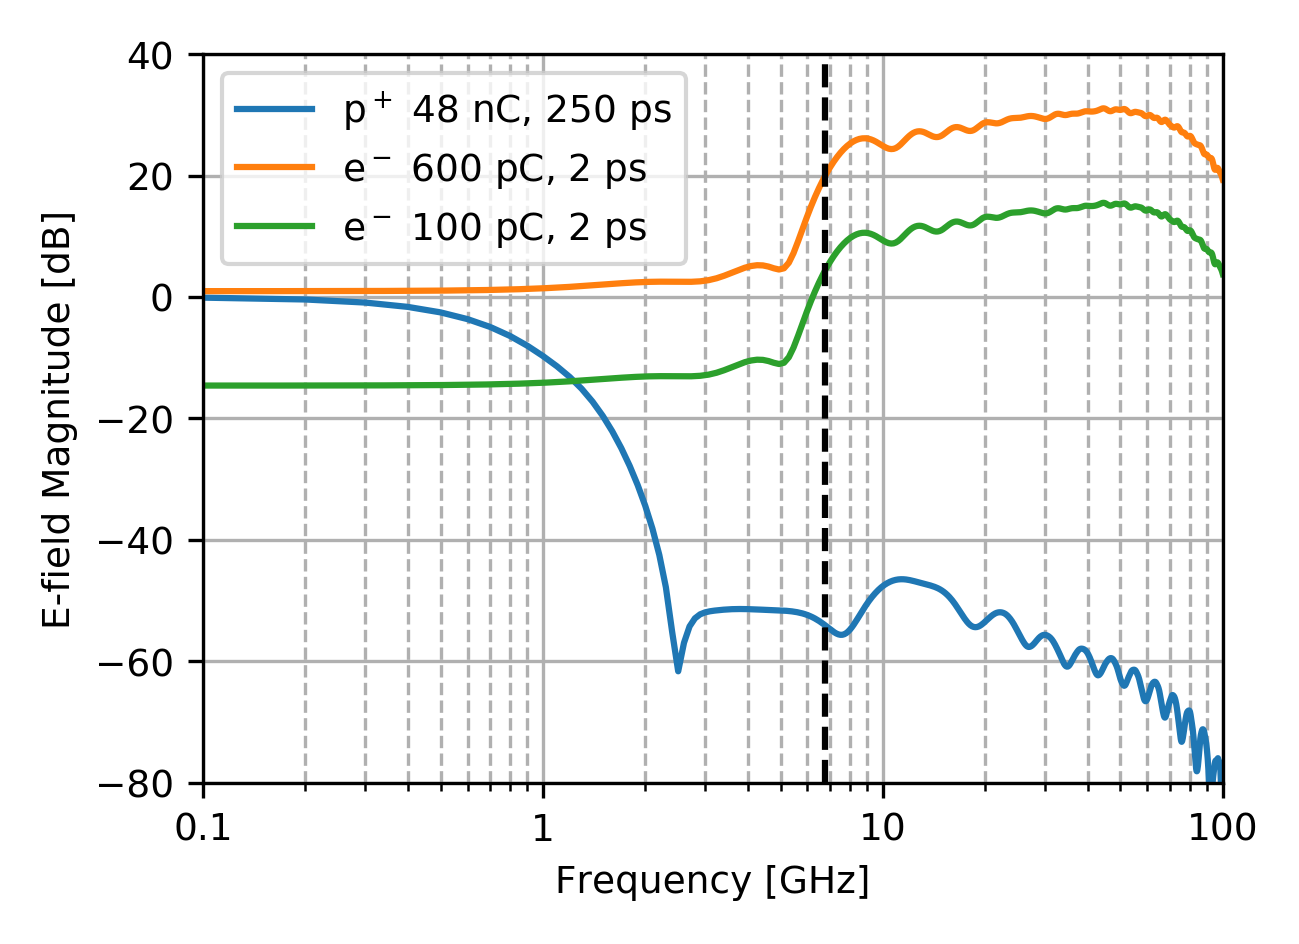
\includegraphics[scale=1, keepaspectratio]{pictures/protons_clear}
\caption{Electric field computed at a probe placed 1~cm above the radiator output surface. Spectra of various beams, as reported in Table~\ref{tab:sim_param_comparison}, are shown. The vertical dashed line is the cutoff frequency of an 18-mm-diameter waveguide loaded with PTFE.}
\label{fig:protons_in_clear}

\vspace{4mm}

\begin{tabular}{l c c c}
\toprule
Name  & Charge & $\sigma$ \\
& nC & ps \\
\midrule
Proton beam			& $48$	  & 250	\\
Electron beam		& $0.6$	  & 2		\\
Electron beam		& $0.1$	  & 2		\\
\bottomrule
\end{tabular}
\captionof{table}{Beam parameters used as baseline parameters for this study. See Table~\ref{awake_all_params:tab} for comparison with the AWAKE operational parameters.} \label{tab:sim_param_comparison}
\end{figure}

The parameters of simulated beams were selected on the one hand to investigate the effect of the AWAKE proton beam on the device tested at CLEAR, and on the other hand to compare them with the CLEAR electron beam. In the case of AWAKE, bunch lengths up to 1~ps are used. However, the simulation results shown in Fig.~\ref{fig:1ps-vs-2} show that, up to 30~GHz, the ChDR emission is not strongly dependent on the simulated bunch length. Studying a 2~ps long bunch was preferred due to the reduced computing time required to complete the simulations.




\begin{figure}[!h]
\centering
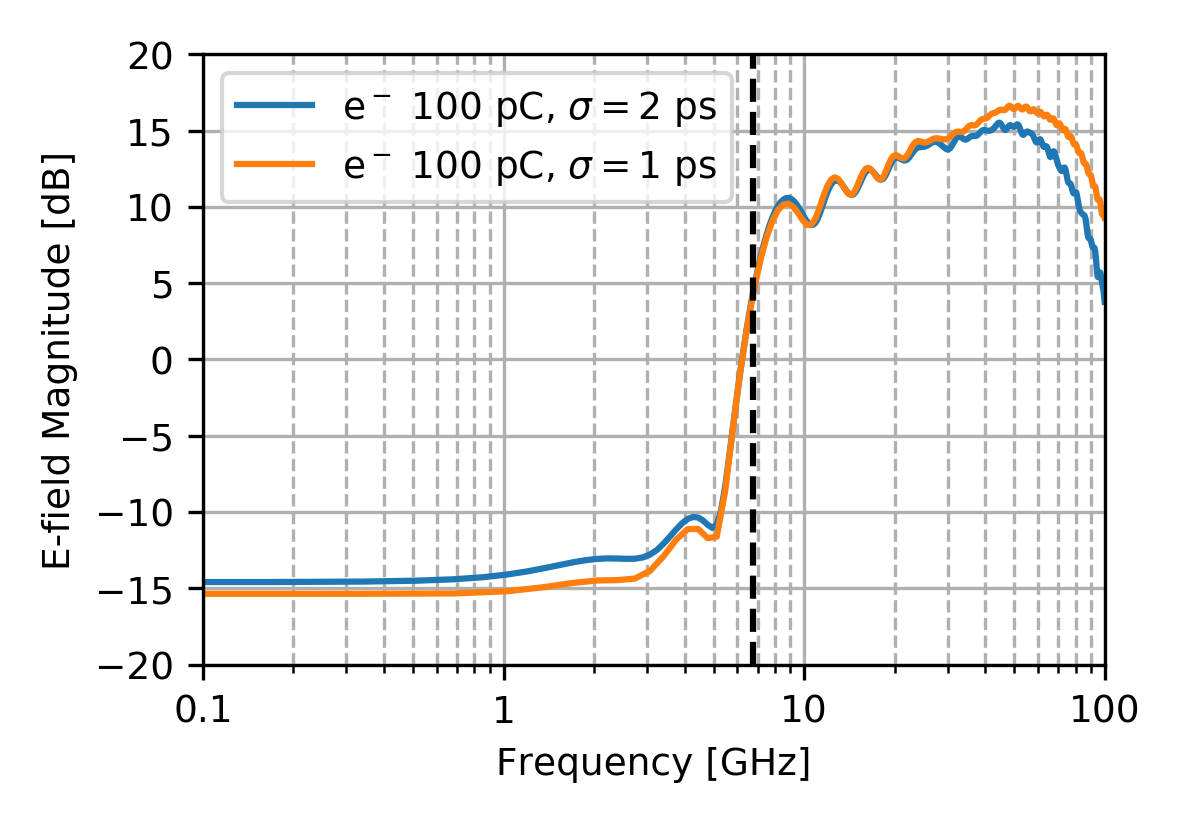
\includegraphics[scale=1, keepaspectratio]{pictures/1ps-vs-2ps}
\caption{Comparison of the electric field spectrum emitted by 1~ps- and 2~ps-long electron bunch with a charge of 100~pC. }
\label{fig:1ps-vs-2}
\end{figure}




\section[Lower-energy beams]{Lower-energy beams}

The AWAKE facility uses a tenfold-lower electron-beam energy compared with CLEAR. Therefore, a different electron-bunch-field distribution is expected, as explained in Chapter~\ref{chapter:copropagating_beams}. The relativistic beam parameters for both facilities are compared in Table~\ref{tab:param_awake_vs_clear}. Although in AWAKE the $\beta$ is still very close to 1, a simulation was performed to assess if the lower beam energy could affect the ChDR emission. The 3D model presented in Section~\ref{sec:single_electrode} was simulated with a 2~ps-$\sigma$ 100~pC electron beam. No appreciable difference in the field spectrum emission was observed, with the maximum differences smaller than 0.01~dB (i.e. 0.1\%).

\begin{table}[!h]
  \centering
    \begin{tabular}{l c c c}
    \toprule
    Accelerator  & Energy & $\gamma$ & $\beta$ \\
    \midrule
    CLEAR & 200 MeV & 392 & 0.999997 \\
    AWAKE & 16 MeV  & 31  & 0.9995\\
    \bottomrule
    \end{tabular}
  \caption{Relativistic electron beam parameters for AWAKE and CLEAR beams.} \label{tab:param_awake_vs_clear}
\end{table}








\section[The design of a vacuum compatible radiator]{The design of a vacuum compatible radiator}

Although the device tested at CLEAR would be sensitive to the electron-bunch position regardless of the proton-bunch presence, some modifications would be necessary before it could be installed in the AWAKE beam line. The test device is not compatible with Ultra-High Vacuum (UHV) and using PTFE in radioactive environments should be avoided due to its rapid degradation~\cite{PTFE:no-vac}. A different radiator material is therefore necessary, which would affect the BPM mechanical design because its permittivity would differ from that of PTFE. Two dielectrics were considered for a vacuum-compatible BPM installed in a radioactive environment: Fused Silica and Alumina 99.5\%. Both change the emission angle of the radiator and the fundamental-mode cutoff frequency. The variation of the Cherenkov angle can be derived from Eq.~\ref{ch_angle}, remembering that $n = \sqrt{\epsilon_r}$ for non-magnetic materials. As the material's relative permittivity increases, so does the Cherenkov angle, up to the maximum value of $90^\circ$. 
On the other hand, the radiator's cutoff frequency decreases if either the material permittivity, or the radiator radius increases (see Eq.~\ref{eq:cutoff_loaded}). Figure~\ref{fig:cutoff_radiators} shows how  the change of the radiator radius affects the radiated electric-field spectrum. The simulations were conducted using the model described in Section~\ref{sec:single_electrode}.
Table~\ref{tab:radiator_materials} presents relevant parameters for the different materials considered. 

\begin{table}[!b]
    \centering
    \begin{tabular}{l c c c}
    \toprule
    Material    & PTFE & Fused Silica & Alumina  \\
    \midrule
    Relative permittivity $\epsilon_r$ & 2.1 & 3.8 & 9.6\\
    Cherenkov angle     $\theta_\text{Ch}$ & $46^\circ$ & $59^\circ$ & $71^\circ$ \\
    Relative cutoff frequency   $f_c/f_\text{c,vac}$    & 0.69 & 0.51 & 0.32\\
    \bottomrule
    \end{tabular}
    \captionof{table}{Relative permittivity of the materials considered for the radiator. The different Cherenkov angles and the fundamental-mode cutoff frequency are reported. The cutoff frequency is normalised to an equivalent evacuated circular waveguide.}
    \label{tab:radiator_materials}
\end{table}


\begin{figure}[!b]
\centering

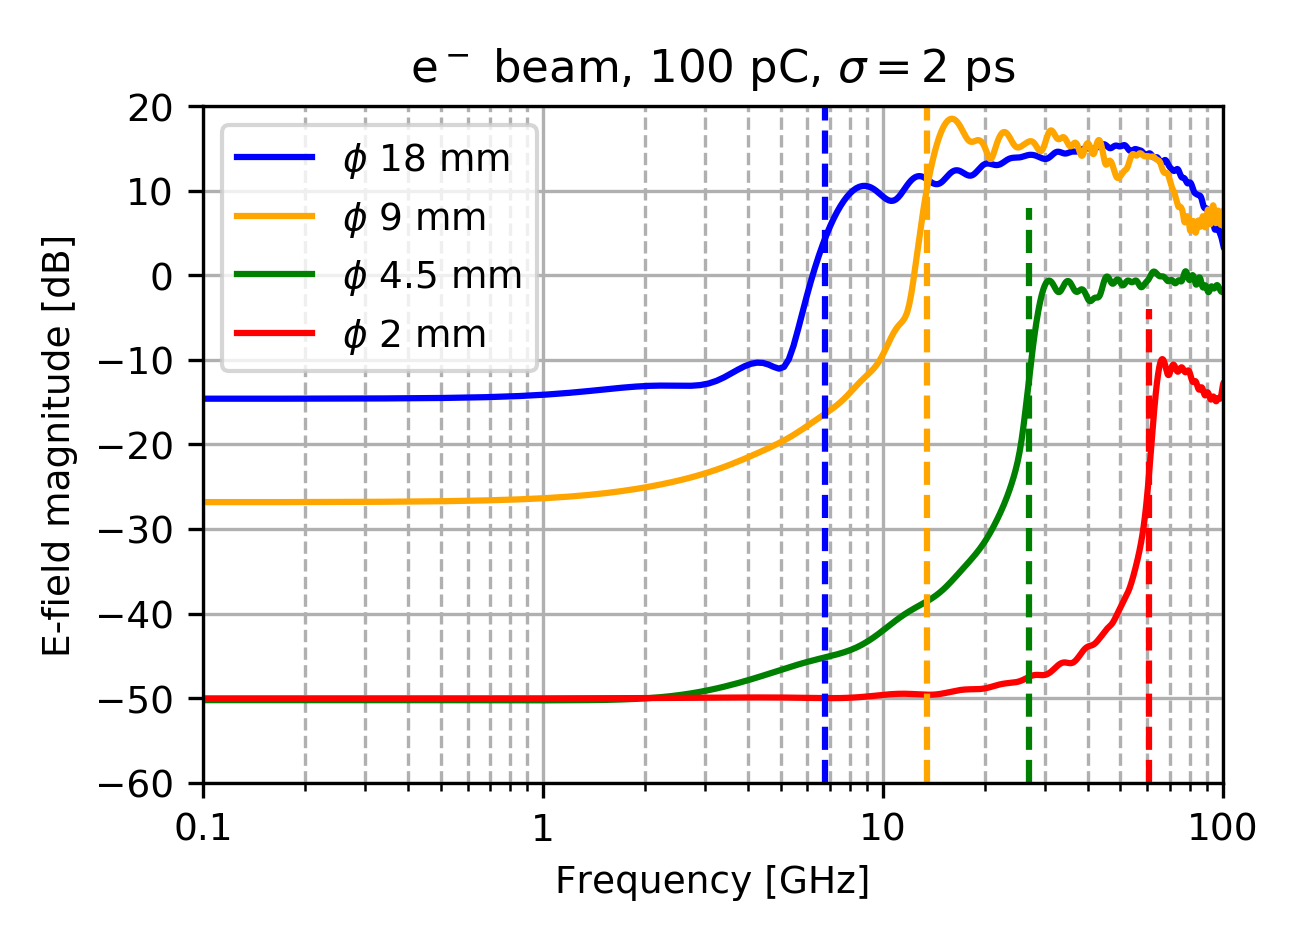
\includegraphics[scale=1, keepaspectratio]{pictures/ptfe_size_scan.png}
\captionof{figure}{Comparison of the electric field vs frequency, measured 1~cm away from the centre of the radiator output surface produced with different radiator radii in a PTFE radiator (model described in Section~\ref{sec:single_electrode}). The coloured vertical dashed lines represent the fundamental mode cutoff frequency of an equivalent PTFE-loaded waveguide of the same diameter (the numerical values are reported in Table~\ref{tab:cutoff_radiators}). }
\label{fig:cutoff_radiators}

\vspace{4mm}

\begin{tabular}{l c c c c c}
\toprule
Diameter (mm)   &  18&9&4.5&3&2\\
$f_c$ (GHz)     &   6.7&13.5&26.9&40.4&60.6\\
\bottomrule
\end{tabular}
\captionof{table}{Fundamental-mode cutoff frequencies for PTFE-loaded waveguides of different diameters.}
\label{tab:cutoff_radiators}

\end{figure}

Based on CERN's experience in realising vacuum-tight assemblies by brazing alumina to metal, the final material of choice is alumina. Compared with PTFE, alumina radiators have a cutoff frequency lower by a factor of~2.15. In order to reach a cutoff frequency in the order of 20~GHz, a 3~mm radiator diameter was selected. See Table~\ref{tab:cutoff_radiators} for a comparison with the cutoff frequency of PTFE radiators of different diameters. The inherent Cherenkov angle for alumina is $71^\circ$.

For an installation in the AWAKE beamline, it is convenient to design the radiators such that they are compatible with the existing BPM vacuum chambers. Such a `dielectric button' consists of a cylindrical metal insert fitted with a vacuum flange. The cylinder is 44~mm long and has a diameter of 36~mm. The alumina radiator is inserted into the cylinder by welding a metal collar brazed to the radiator. The cylinder dimensions allow one to accommodate radiators with diameters up to 15~mm, while retaining the $71^\circ$ angle. Figure~\ref{fig:body_button} shows an existing BPM vacuum chamber with the dielectric button inserted, and details of the button. 


An alternative design option featuring an orthogonal radiator to the\linebreak beampipe was also considered. This design with the radiator at $90^\circ$ would provoke internal reflections which could result in signal deterioration, while offering a significantly simpler construction. 




\begin{figure}[!b]
\centering
\subfigure[BPM body]
  {\includegraphics[width=6.5cm, keepaspectratio]{pictures/awake_body}}
\hspace{3mm}
\subfigure[Button detail]
  {\scalebox{-1}[1]{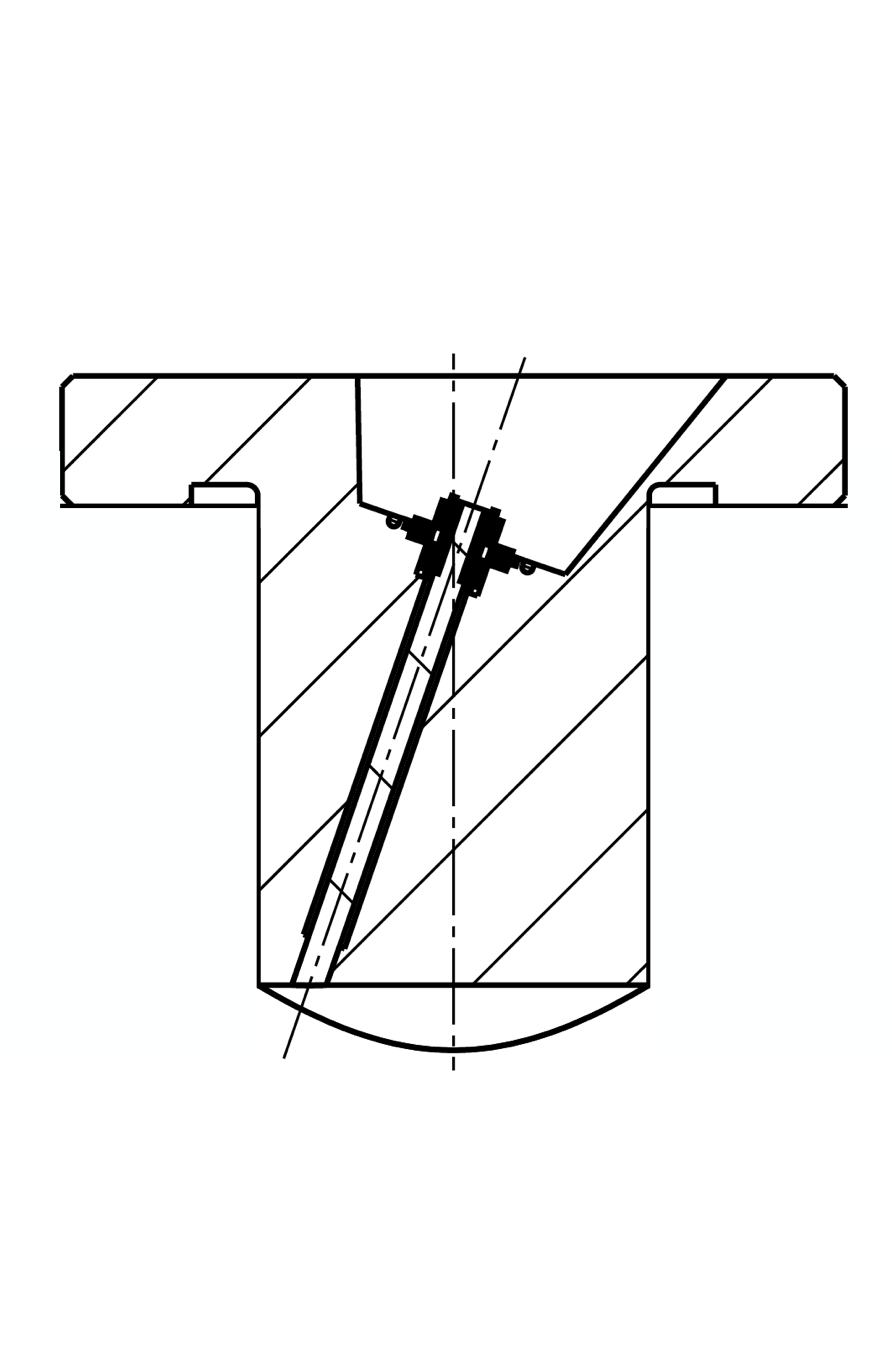
\includegraphics[width=6.5cm, keepaspectratio]{pictures/AWAKE_button}}}
\caption{Longitudinal section of the BPM vacuum chamber (on the left) and of the dielectric button (on the right). The beam direction is right to left. The design is preliminary.}
\label{fig:body_button}
\end{figure}

In general, the design is substantially more complicated than the CLEAR test device described in Chapter~\ref{chapter:CLEAR_test}, which featured radiators with a diameter of 18~mm and an average length of 25~mm. In the AWAKE case, the diameter is reduced to 3~mm while the length is increased to 40~mm. While in the CLEAR test device the radiation fronts not propagating at the Cherenkov angle quickly reach the output surface with limited reflections, this is no longer true in the AWAKE design. Therefore, part of the radiation would be subjected to multiple reflections and eventually some would be reflected back into the beampipe. An additional complication is the increased electromagnetic-simulation complexity due to the longer radiator.








\section[Radiator oriented at the Cherenkov angle]{Radiator oriented at the Cherenkov angle}\label{sec:future_radiator_71}

The design of a ChDR radiator oriented at the Cherenkov angle offers the simplest field-propagation dynamics. In fact, the ChDR front is not reflected inside the radiator as it propagates on axis. Conversely, the DR fronts are not emitted on axis, and therefore may be reflected during the propagation before reaching the exit surface.

A 3D electromagnetic model was created to simulate this configuration using an average radiator length of 7~mm. Although the radiator size for a real-life BPM would be in the order of 40~mm, a shorter radiator was simulated to reduce the computing power required. Furthermore, a heavily optimised meshing was necessary to limit the simulation complexity due to the relatively large mechanical dimensions. The approach was similar to what was done for the CLEAR test device in Section~\ref{sec:single_bunch}. Figure~\ref{fig:71deg_model} shows the 3D model and its division into separate meshing regions. High resolution meshing of 20 cells per wavelength was used in regions 1, 5 and 6. A 100~pC, 2~ps-long electron bunch was used as an EM source.

The emitted electric field was computed for a probe placed 1~cm above the center of the output surface. The simulated cutoff frequency for a 3~mm diameter radiator matched the theoretical value of 19.11~GHz. Additional simulations were carried out to assess the effect of slight angle variations due to mechanical tolerances. This would be equivalent to a slight change of the dielectric constant of the radiator material. The comparison of the emitted spectrum for $\pm1^\circ$ variations from the Cherenkov angle of $71^\circ$ is shown in Fig.~\ref{fig:alumina_cutoff}. In general, a discrepancy up to 1~dB is observed below the fundamental mode cutoff frequency and up to 0.2~dB above it. 

Choosing a high dielectric constant material for the radiator is particularly favourable as the Cherenkov angle is not very sensitive to dielectric constant variations. For high-purity alumina (99.5\%), the dielectric constant $\epsilon_r=9.4$ results in a Cherenkov angle of $71^\circ$. Even rather large $\epsilon_r$ variations, for example $\epsilon_r = 9$ and $\epsilon_r = 10$ result in limited variations of the Cherenkov angle of $70.5^\circ$ and $71.6^\circ$, respectively. This is reassuring for two reasons: first, it is not necessary to adapt the radiator installation angle to the exact value of the radiator dielectric constant; secondly, although the dielectric constant has a frequency dependence, it is typically low enough that it would not affect the emission angle of the different spectral components. This approximation is justified up to approximately 100~GHz, but it is not necessarily true at higher frequencies where $\epsilon_r$ can drastically change~\cite{epsilon_r_THz}.

\begin{figure}[!t]
\centering
\subfigure[Model overview]
  {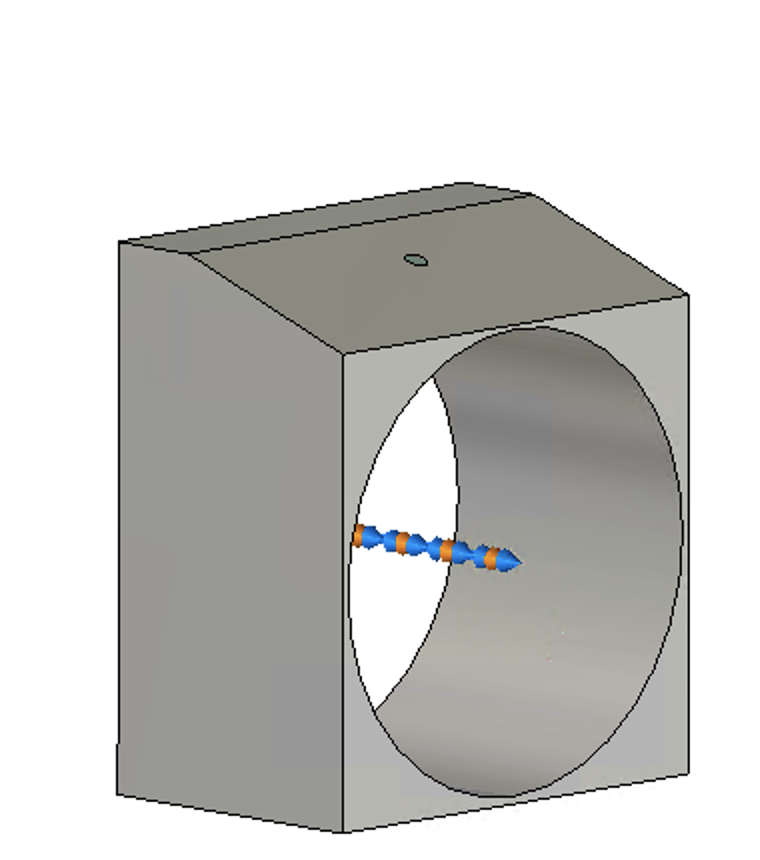
\includegraphics[width=6.5cm, keepaspectratio]{pictures/71deg_novac}}
\hspace{3mm}
\subfigure[Meshing regions]
 {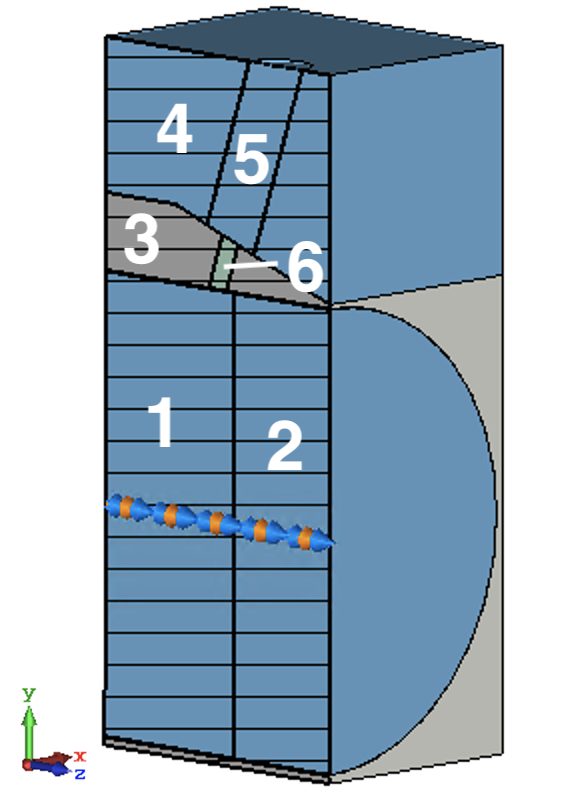
\includegraphics[width=6.5cm, keepaspectratio]{pictures/71deg_7mm}}
\caption{(a) Simulated model overview and (b) meshing regions. The vacuum volumes in (a) are not shown. Coarse mesh size is used for the metal (3), and the vacuum regions (2 and 4). The finely meshed regions are the initial part of the beampipe (1), the radiator (6) and the vacuum above the radiator (5). For reference see Section~\ref{sec:single_bunch}.}
\label{fig:71deg_model}
\end{figure}





\begin{figure}[!t]
\centering
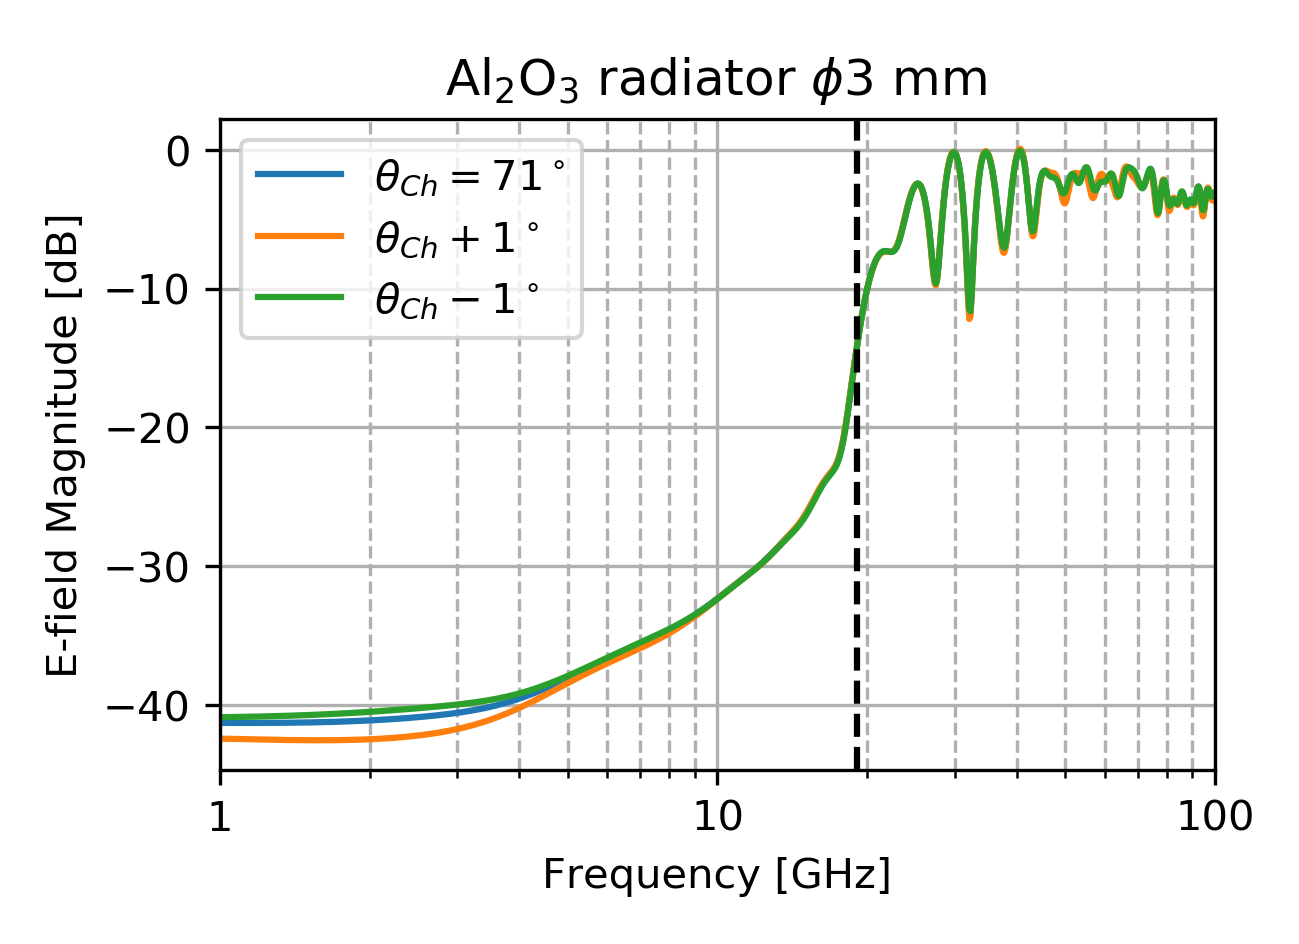
\includegraphics[scale=1, keepaspectratio]{pictures/Alumina_3mm_1cm_above_center_normalised}
\caption{Electric field 1~cm away from the radiator output surface versus frequency. The results for a radiator orientation at $71\pm1^\circ$ are shown. The dashed black line marks the theoretical cutoff frequency of $19.1$~GHz.} \label{fig:alumina_cutoff}

\end{figure}










\section[Radiator orthogonal to the beampipe]{Radiator orthogonal to the beampipe}

Other than the nominal Cherenkov angle, an AWAKE ChDR BPM could also use radiators orthogonal to the beam propagation direction. Although such a design could be simpler to construct, it would potentially lead to internal reflections of the emitted wavefronts that must considered. 



\subsection[Simulation]{Simulation}

A 3D electromagnetic simulation model was developed similar to the one with radiators oriented at the Cherenkov angle described in Section~\ref{sec:future_radiator_71}. A vertical radiator with a 7~mm average length and a 3~mm diameter was placed in a metal beampipe. Again, a regional meshing approach was used. Figure~\ref{fig:90deg_model}~(a) shows the simulated 3D model and how it was divided into the different meshing regions. The finely-meshed regions 1, 5 and 6 used 20 mesh cells per wavelength. A 100~pC 2~ps-long electron bunch was used as a source. Figure~\ref{fig:90deg_model}~(b) shows the computed electric field on the longitudinal-cut plane. 

The substantially different field-propagation evolution in a radiator not oriented at the Cherenkov angle is illustrated in Fig.~\ref{fig:90deg_propagation}, showing the radiator and the surrounding vacuum. In~(a) and~(b), the bunch has just passed the radiator surface, and several wavefronts are visible in the radiator. When the radiation reaches the output surface in~(c), the first fronts are emitted towards the right, while the subsequent fronts in ~(d) propagate towards the left. Additionally, some wavefronts in~ (e) are internally reflected inside the radiator and in~(f) propagate back to the beampipe. These results suggest that, for long radiators, different wavefronts may interfere with each other which could lead to a different spectrum of emission from the radiator compared with the radiator installed at the nominal Cherenkov angle. 

The beam position sensitivity of the two designs was compared by considering the absolute value of the electric field in the time domain computed for a probe at the centre of the output face using methods described in Section~\ref{sec:position_sensitivity}. The beam-position sensitivity over a 6~mm range is shown in Fig.~\ref{fig:90deg_vs_71deg}. No appreciable difference can be observed. 





\begin{figure}[!t]
\centering
\subfigure[]
  {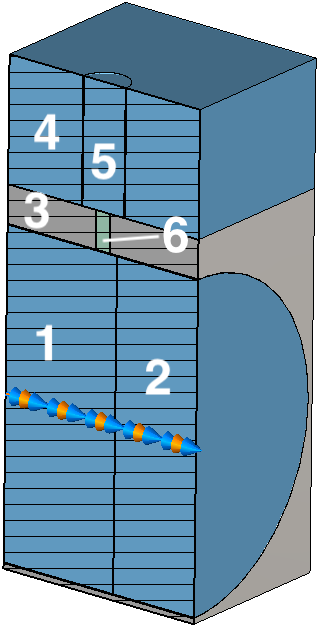
\includegraphics[width=4.5cm, keepaspectratio]{pictures/90deg_cut}}
\hspace{8mm}
\subfigure[]
 {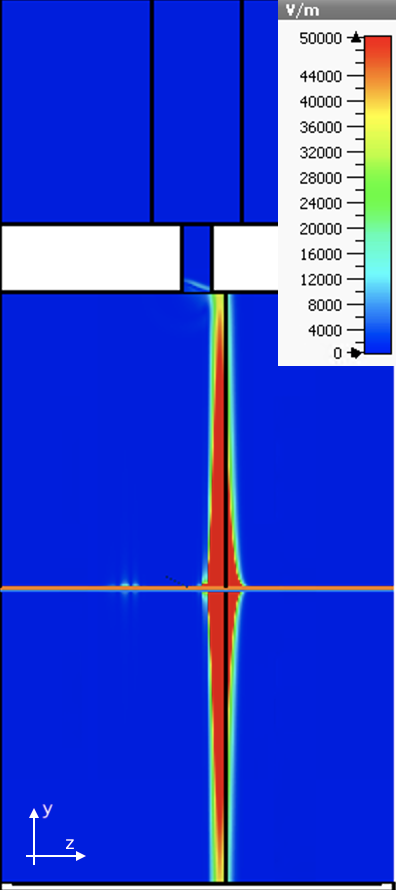
\includegraphics[width=3.9cm, keepaspectratio]{pictures/field90_1}}
\caption{(a) Simulated model with the meshing regions indicated and (b) the absolute value of the electric field in the transverse plane. Minimum resolution is used for the metal (3), and the vacuum regions (2 and 4). The high quality meshing regions are the initial part of the beampipe (1), the radiator (6) and the vacuum above the radiator (5). See for reference Section~\ref{sec:single_bunch}. The simulation was produced with a bandwidth of 100~GHz, and a 100~pC and 2~ps-long electron beam.}
\label{fig:90deg_model}
\end{figure}





\begin{figure}[!h]
\centering
\subfigure[t $=110$ ps]{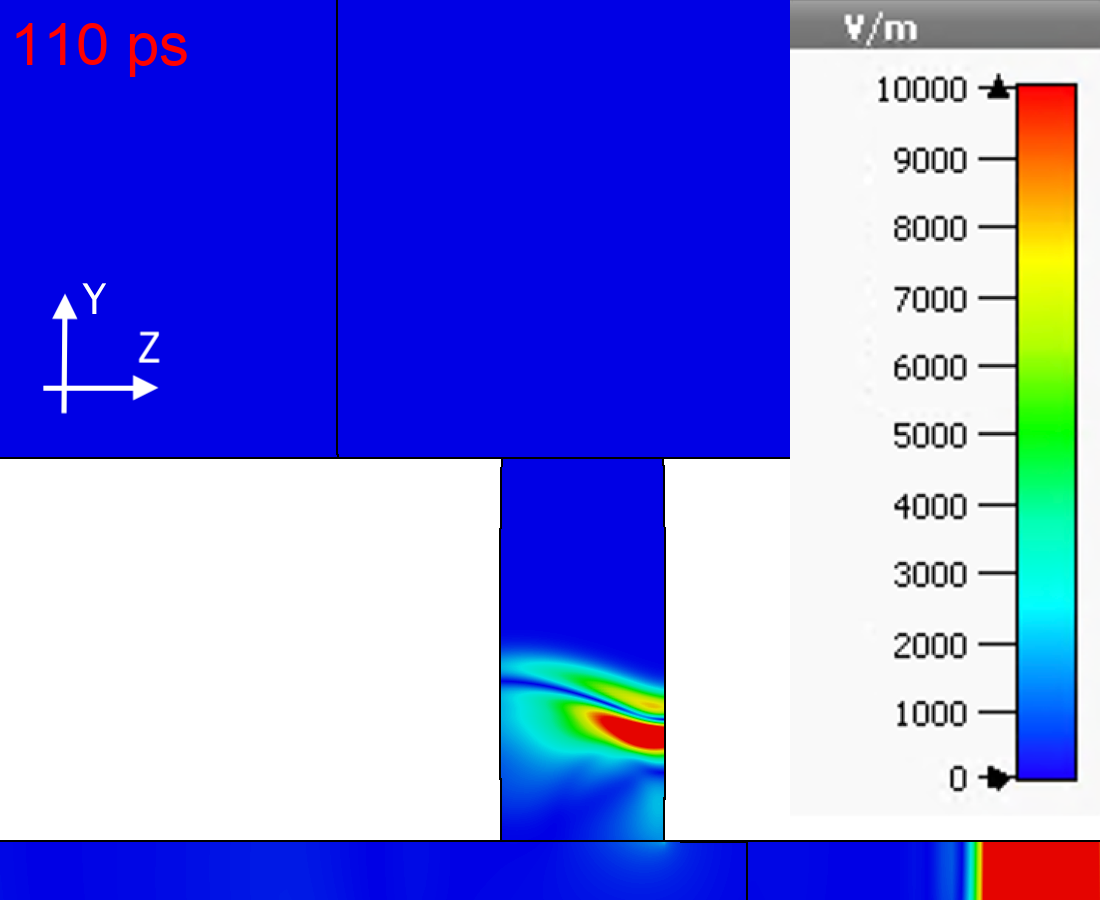
\includegraphics[width=4.3cm, keepaspectratio]{pictures/90deg_1}}
\hspace{1mm}
\subfigure[t $=122$ ps]{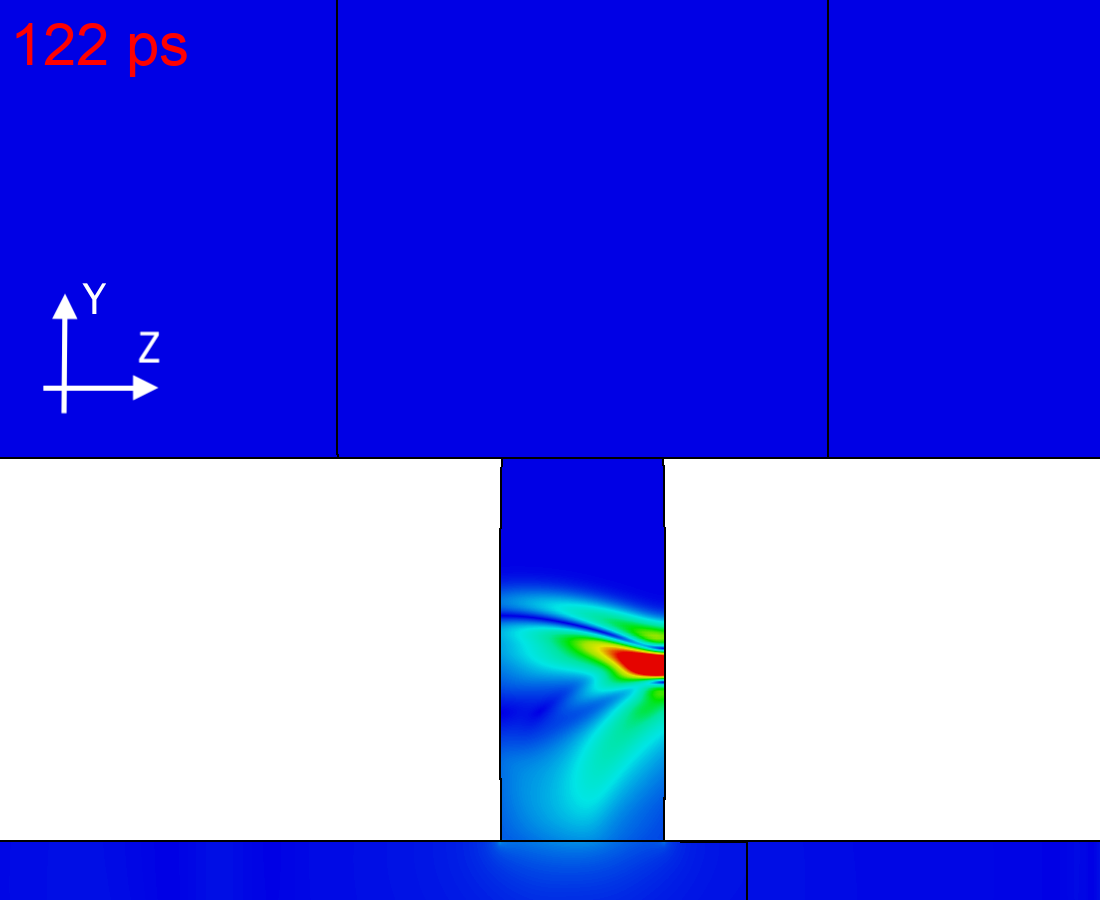
\includegraphics[width=4.3cm, keepaspectratio]{pictures/90deg_2}}
\hspace{1mm}
\subfigure[t $=162$ ps]{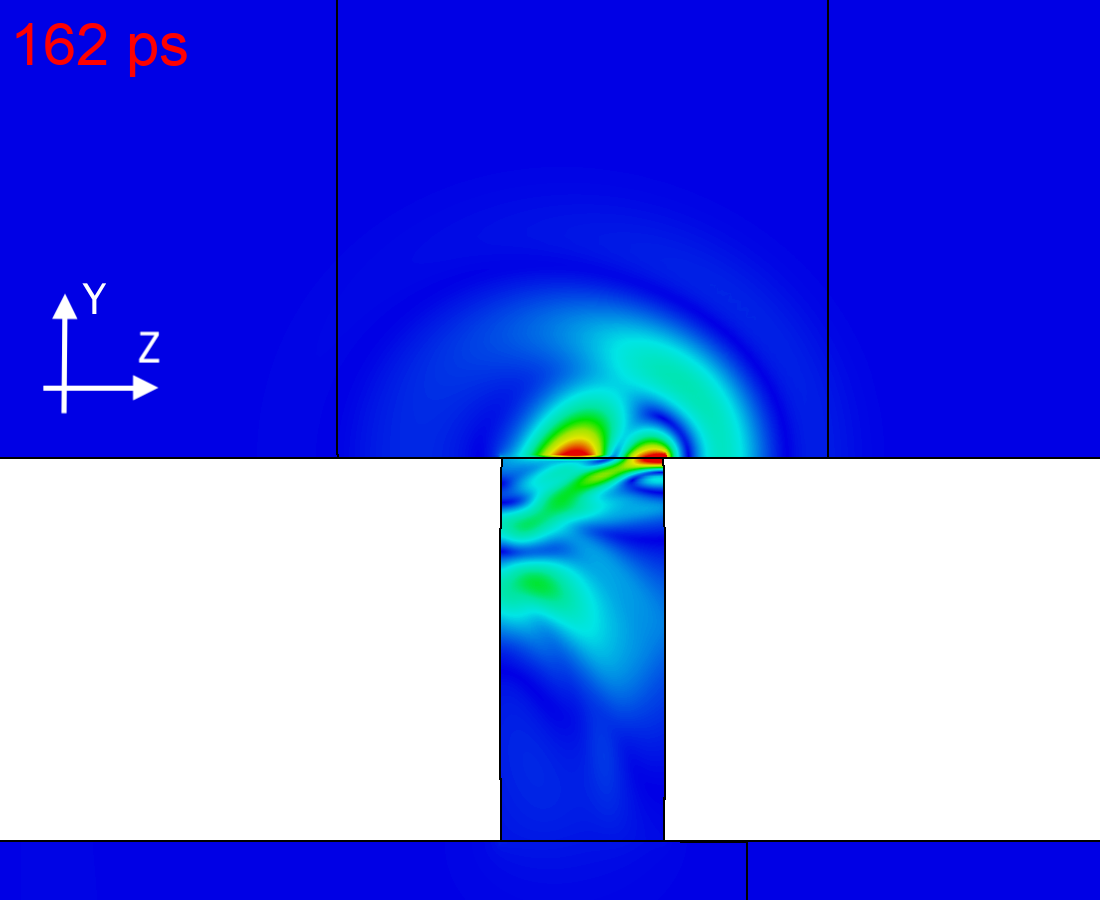
\includegraphics[width=4.3cm, keepaspectratio]{pictures/90deg_3}}\\

\subfigure[t $=182$ ps]{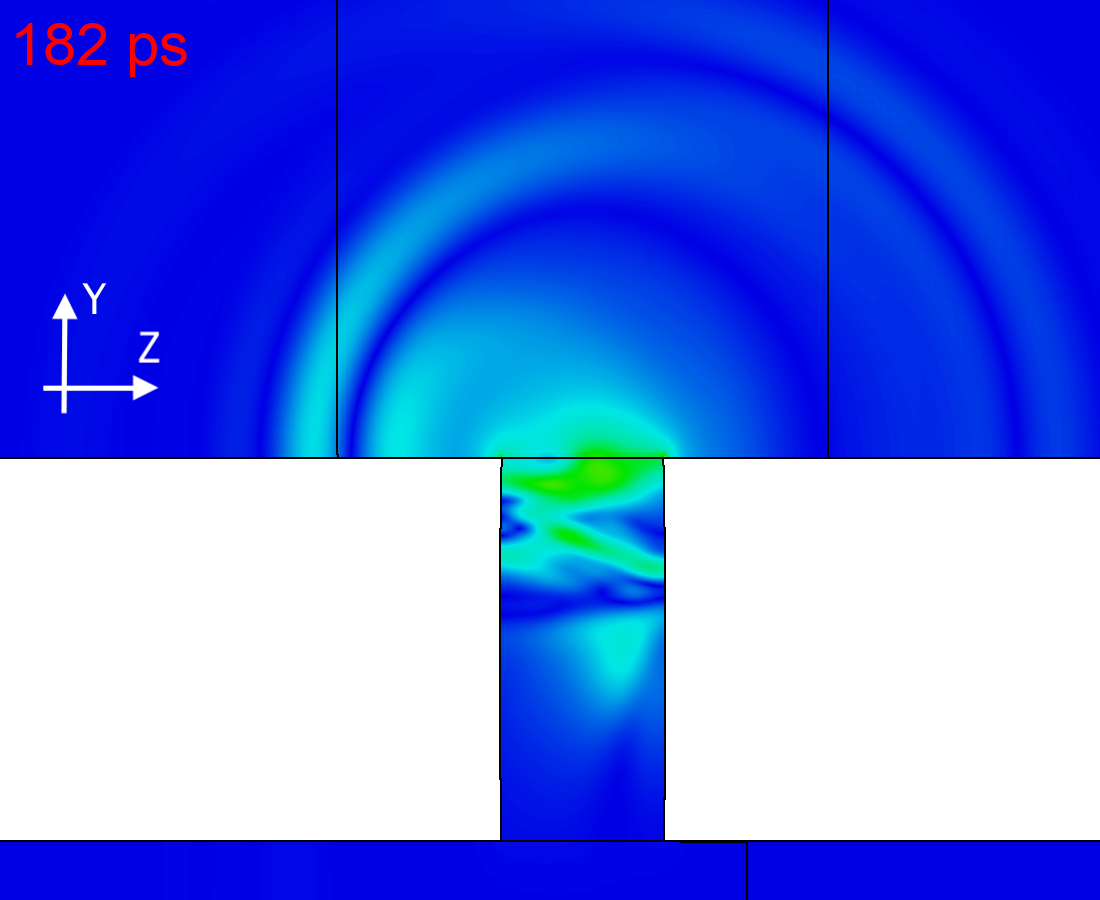
\includegraphics[width=4.3cm, keepaspectratio]{pictures/90deg_4}}
\hspace{1mm}
\subfigure[t $=222$ ps]{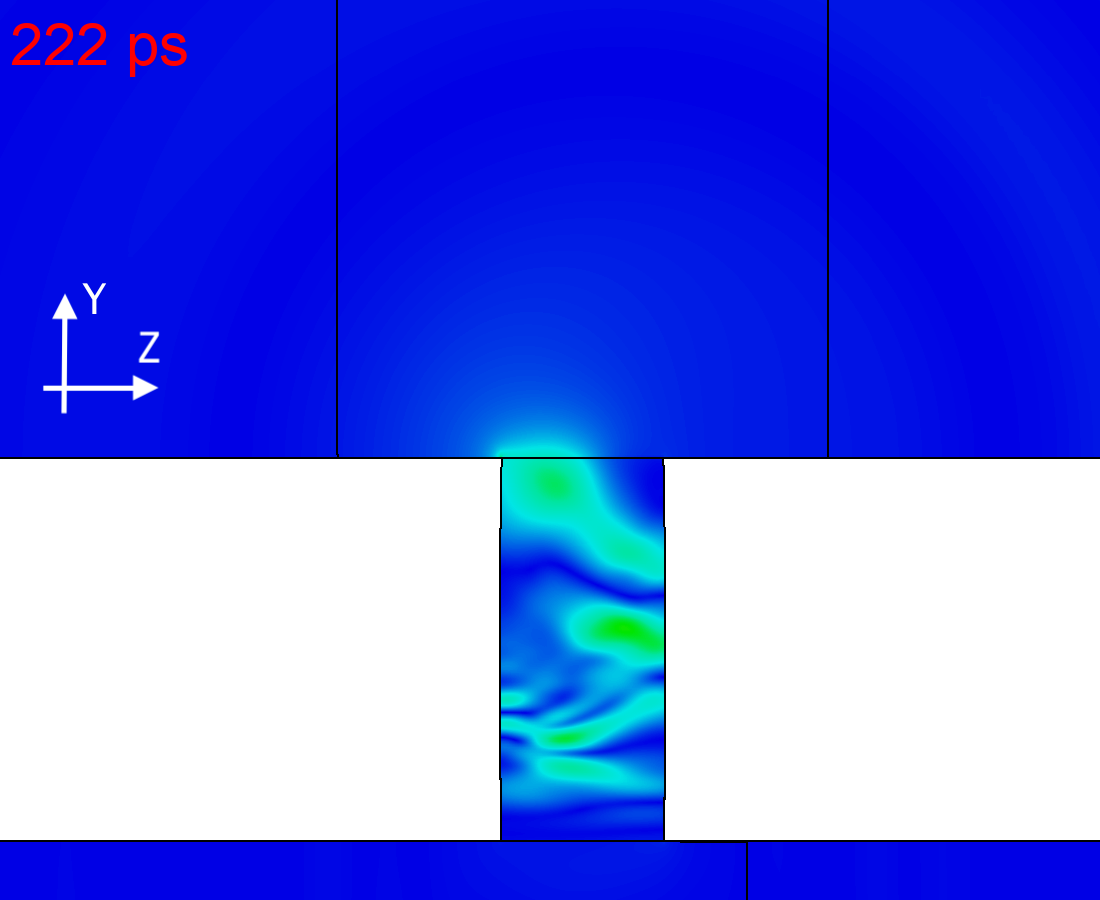
\includegraphics[width=4.3cm, keepaspectratio]{pictures/90deg_5}}
\hspace{1mm}
\subfigure[t $=252$ ps]{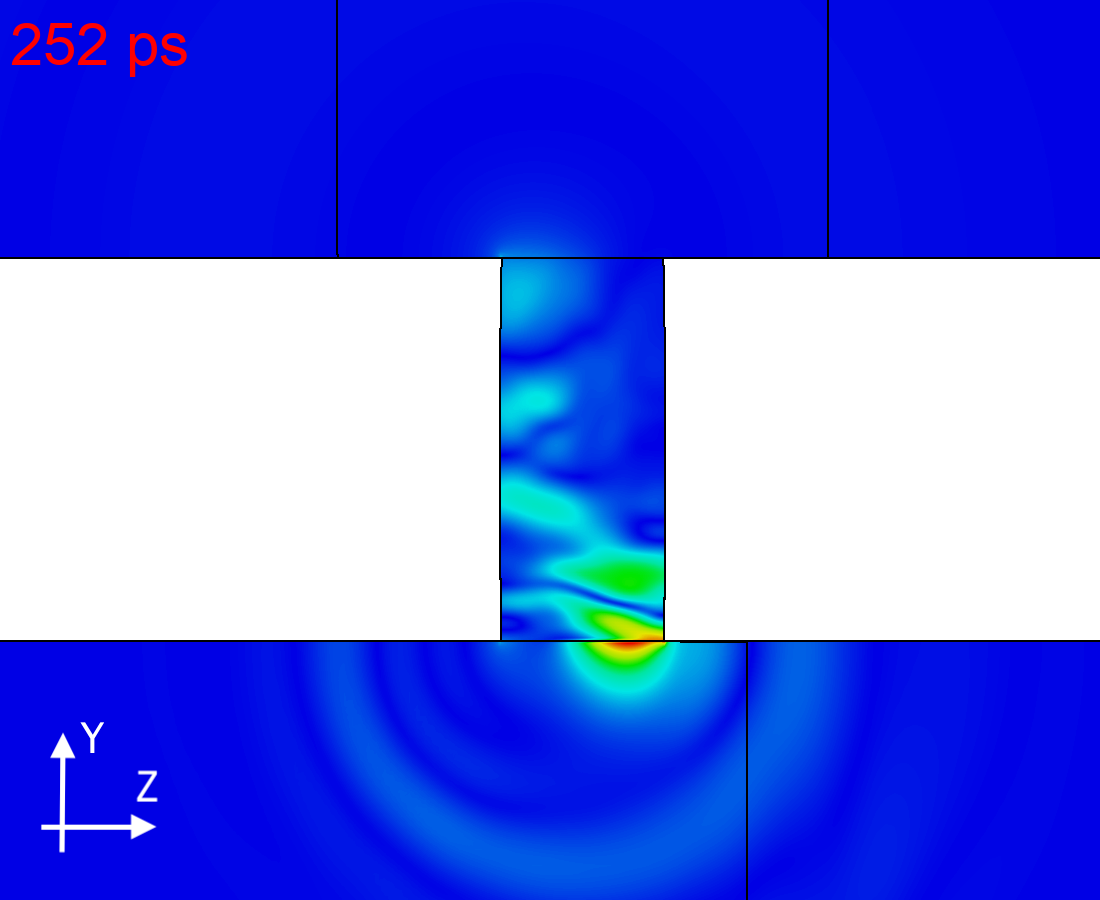
\includegraphics[width=4.3cm, keepaspectratio]{pictures/90deg_6}}

\caption{Absolute value of the electric field in the radiator and in the vacuum outside the vacuum pipe (on top). The field is displayed at different times. The internal reflection of the wavefronts can be seen in (b) and (c). At the exit of the radiator, two fronts propagating in different directions are visible in (d). Due to the medium change, a part of the radiation is also sent backwards to the beampipe as shown in (f).}
\label{fig:90deg_propagation}

\vspace{3mm}
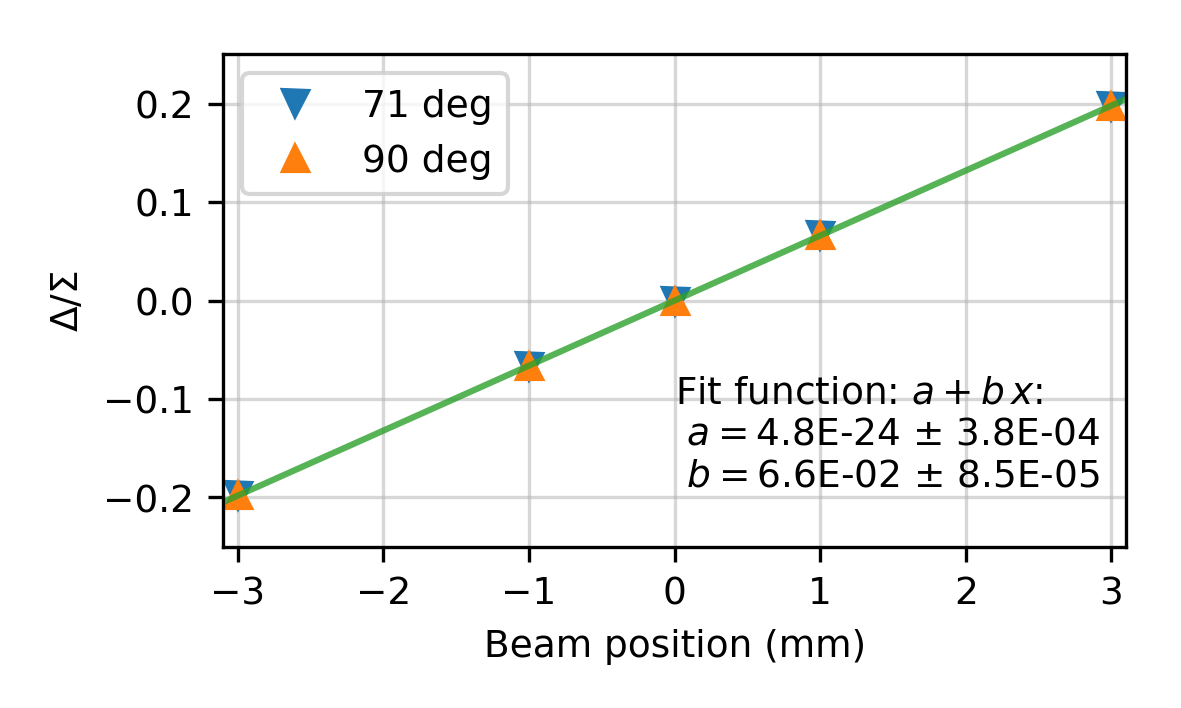
\includegraphics[scale=1., keepaspectratio]{pictures/90vs71}
\caption{Comparison of the beam position sensitivity of radiators oriented at 71 and 90 degrees. The green line shows the linear fit, which exhibit the same response for both the orientations.}
\label{fig:90deg_vs_71deg}

\end{figure}




\newpage

\subsection[Experience with orthogonal waveguide coupling]{Experience with orthogonal waveguide coupling}

The CLEAR facility is equipped with a device that is conceptually similar to an orthogonal ChDR pickup. Although this device was built with a different purpose and without considering the ChDR emission, it is instructive to consider the signal produced by such a device. 

The BPRW \cite{BPRW:linac2010} is an RF pickup that consist of a standard WR28 (Ka~band) rectangular waveguide connected orthogonally to the beampipe. A vacuum tight connection between the vacuum pipe and the waveguide is obtained using an alumina window. This device was designed to perform a relative measurement of the bunch compression in the CTF3 facility \cite{CTF3} by producing a signal proportional to the bunch length \cite{Lefevre:2008zz}. The BPRW uses the fact that the high-frequency components of a shorter bunch are more intense than those of a longer bunch and therefore couple out more strongly through the waveguide. 

Based on current understanding of Cherenkov Diffraction Radiation, it can be assumed that a ChDR front is produced in the BPRW alumina window when a beam passes in its proximity. Besides the ChDR front, there are also a number of DR fronts due to the electromagnetic discontinuities. To study the signals produced by the BPRW, the Ka-band RF detection system previously used to measure the beam-position sensitivity of the ChDR test device in the horizontal plane was employed. One of the diodes was left in place on the test device to detect its ChDR emission, while the other one was installed at the BPRW port after a short waveguide which provided some physical distance between the diode and the beam to avoid any radiation damage. The same attenuation of 30~dB was used in both cases. Figure~\ref{fig:bprw} shows the BPRW port with one of the Ka-band detectors installed.

The signals from the BPRW and the ChDR test device are compared in Fig~\ref{fig:bprw_vs_chdr}. The signals are arbitrarily scaled, as their ratio depends on a number of factors such as the beam position along the beamline, the signal-transmission efficiency and the alignment of the devices. It is nevertheless evident that the signals produced by the ChDR and the BPRW are different. The pulse produced by the ChDR test device is significantly shorter. Therefore, it can be speculated that the BPRW is not suitable for measurements of bunch trains. The allocated experimental beam time was not sufficient to test if a correlation between the BPRW signal and the beam position exists. 

\begin{figure}[!t]
\centering
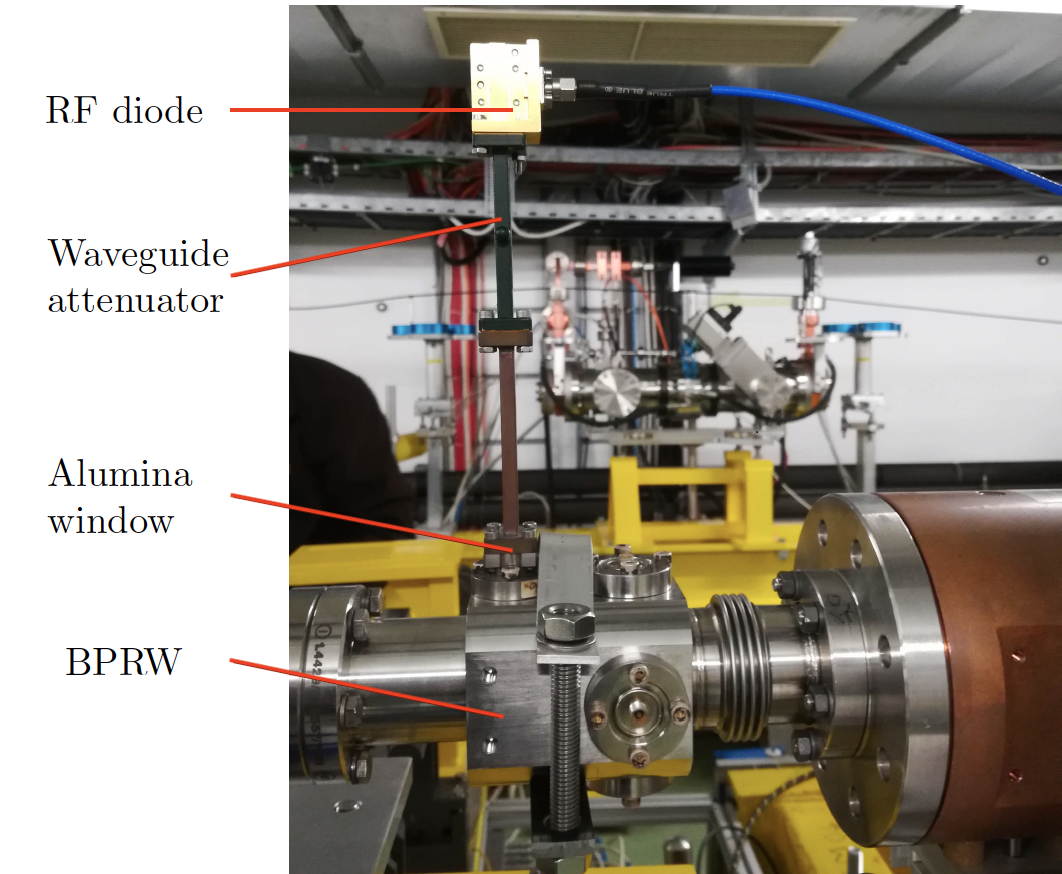
\includegraphics[width=10cm, keepaspectratio]{pictures/BPRW_diode_caption}
\caption{Diode detector installed on a BPRW port. In order from the beampipe: the alumina window assembly is the grey metallic part, then a copper waveguide straight section, a green 30~dB waveguide attenuator and the Schottky diode detector.}
\label{fig:bprw}

\vspace{5mm}

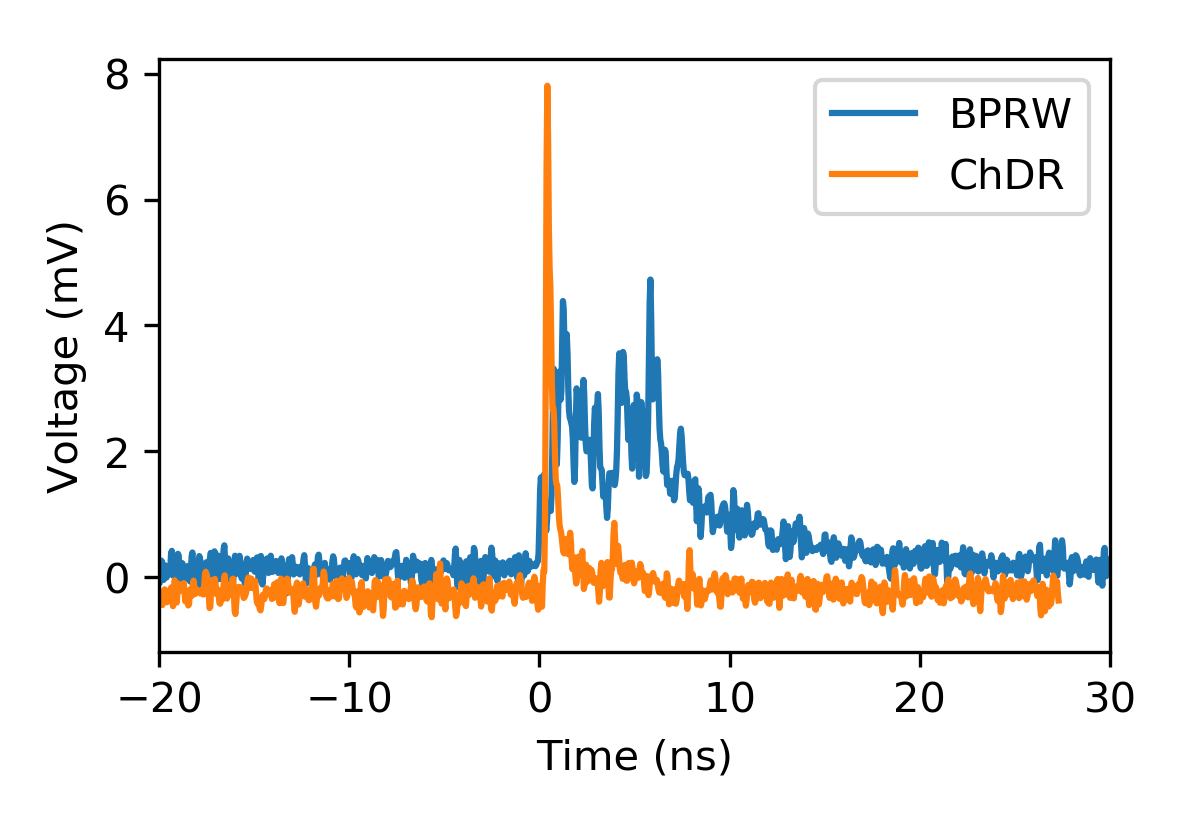
\includegraphics[scale=1,keepaspectratio]{pictures/bprw_vs_chdr}
\caption{Diode detector output voltage for a BPRW and a ChDR radiator. The signals are arbitrarily scaled. The figure shows the different length of the two signals.}
\label{fig:bprw_vs_chdr}
\end{figure}








%%%%%%%%%%%%%%%%%%%%%%%%%%%%%%%%%%%%%%

\newpage



\section[Future developments for ChDR BPMs]{Future developments for ChDR BPMs}\label{sec:fd_chBPM}

The ChDR emission is a very promising novel technique for beam position measurements. However, realising a vacuum-compatible device poses a number of engineering challenges. In particular, the use of high permittivity materials results in radiators with diameters of the order of a few millimetres making the mechanical design challenging.

A preliminary vacuum-tight design is illustrated in Fig.~\ref{fig:new_button}. The radiator is inserted in a metal cylinder featuring a standard vacuum flange to be fixed to the BPM body. The radiator's beam-facing surface is flush with the beampipe. The radiator air-side surface is flat and orthogonal to the radiator axis. To assure vacuum tightness the radiator is brazed with a metal collar close to the output surface. The collar can then be welded to the metal housing. 


\begin{figure}[!b]
\centering
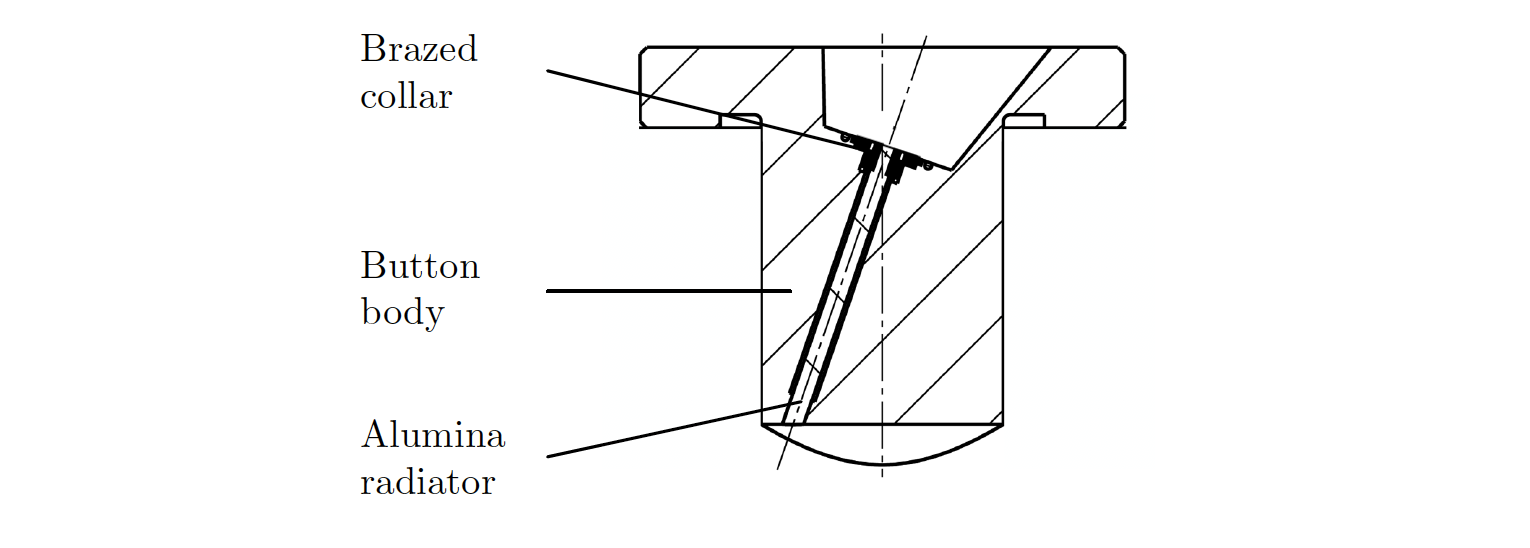
\includegraphics[width=14cm, keepaspectratio]{pictures/button_detail}
\caption{A preliminary design of a vacuum-tight dielectric insert for a ChDR BPM.}
\label{fig:new_button}
\end{figure}

A transition piece attached to the radiator output surface has to be designed to couple the device to a standard waveguide connected to a detection system operating at the desired frequency. 

Extensive additional work is necessary to assess the impact of the internal reflections on the produced signals. Electromagnetic simulations can be improved using resistive metals and dispersive dielectrics in place of perfect materials. Some optimisation of the developed simulation models may be necessary to estimate the absolute power levels generated by the radiator.



\section[The AWAKE ChDR BPM system]{The AWAKE ChDR BPM system}\label{sec:fd_AWAKE}

The present BPM layout in the AWAKE beamline is shown in Fig.~\ref{fig:awake_layout_fd} alongside a modified version with three ChDR BPMs installed. After the proposed modifications, the AWAKE beamline has to maintain an independent proton BPM system (pBPM) to measure the proton beam trajectory from the extraction in the SPS to the beam dump after the plasma cell. The existing electron BPM system (eBPM) is also proposed to be maintained to measure the electron beam trajectory when no proton beam is present. The ChDR BPMs are added to measure the electron beam position when the proton beam is also present and their impact on the other systems should be minimised. Such integration is challenging due to the limited beamline space available in AWAKE. The AWAKE ChDR BPM mechanical design must take into account the beamline integration constraints. Moreover, the RF front-end and acquisition electronics would also need to be developed from scratch in order to deliver an operational system. 


Two ChDR BPMs are foreseen for the common beamline, before the plasma cell. They are installed at the largest distance apart possible to increase the electron beam pointing resolution in the plasma cell. The first BPM is placed immediately after the merging point of the electron and proton beamlines. The second BPM replaces the standard pBPM closest to the plasma cell. The BPM conversion could be achieved by replacing the electrostatic buttons into ChDR buttons (See items number 1 and 3 in Fig.~\ref{fig:awake_layout_fd}) if the ChDR buttons are designed to fit the existing pBPM body.

To retain the total number of pBPMs in the common beamline, the adjacent eBPM could be converted to measure both the proton and the electron beams (See item number 2 in Fig.~\ref{fig:awake_layout_fd}), e.g. by splitting the eBPM output signal, sending the output signal to the eBPM electronics (to measure the electron position in absence of protons) and to the pBPM electronics that belonged to the converted pBPM (item 1 in Fig.~\ref{fig:awake_layout_fd}). Such a modification may require some additional analogue signal conditioning. However, while this approach maintains the total number of proton BPM, it also reduces the resolution of the split eBPM, the impact of which has to be estimated. 

One of the main design challenges described in Chapter~\ref{chapter:copropagating_beams} is the apparent non-reproducibility of the proton beam spectrum leading to shot-by-shot variations in the ratio of proton and electron bunch powers. As the streak camera measurements were not conclusive, additional measurements are necessary to estimate the the real proton beam spectrum. If the proton beam power in the ChDR BPMs detection band is significant compared to the electron beam power, and it is fluctuating shot-by-shot, it could be measured by using a dedicated device (item 4 in Fig.~\ref{fig:awake_layout_fd}). This device, installed in the proton beamline, is a ChDR BPM in which the the four electrodes signals are used to estimate the proton bunch power in the detection band. To be independent from the beam position, the four signals can be summed. Such an approach is commonly used in longitudinal profile monitors. 

The described setup would make it possible to reconstruct the electron beam position in presence of a more intense proton beam. In case of an excessive proton beam signal fluctuation in the ChDR BPM detection band, the whole instrumentation pool can be used to correct the measurements for the proton beam position. However, the necessity for such correction has to be assessed with measurements once the proton beam is available during the next run.


\clearpage
\begin{landscape}
\begin{figure}
\centering
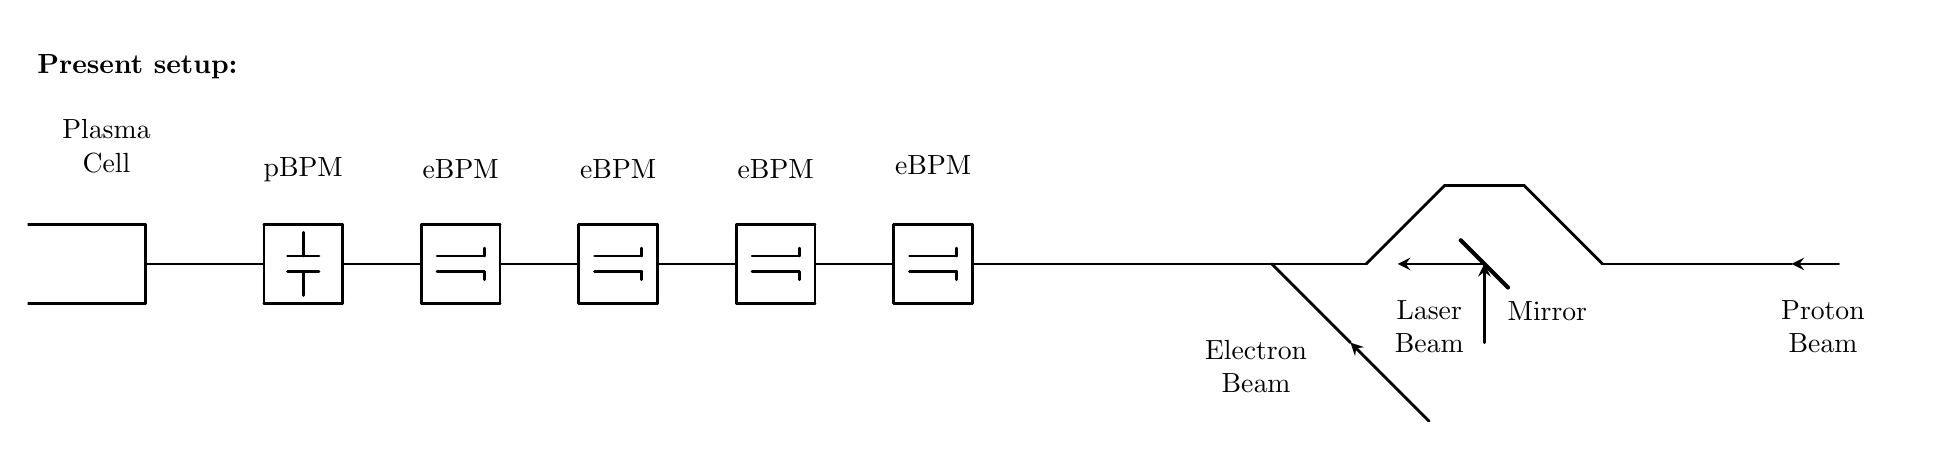
\begin{tikzpicture}[line cap=round,line join=round,>=stealth,x=1cm,y=1cm]
% new version
\clip(-10,-2) rectangle (14, 3);
\draw (-10.,2.5) node[anchor=west] {\textbf{Present setup:}};
\draw [line width=1pt] (-10,0.5)-- (-8.5,0.5);
\draw [line width=1pt] (-8.5,0.5)-- (-8.5,-0.5);
\draw [line width=1pt] (-8.5,-0.5)-- (-10,-0.5);
\draw (-9.,1.5) node[anchor=center] {\parbox{4cm}{\centering Plasma\\Cell}};
\draw [line width=1pt] (-7,0.5)-- (-7,-0.5);
\draw [line width=1pt] (-6,-0.5)-- (-6,0.5);
\draw [line width=1pt] (-6,0.5)-- (-7,0.5);
\draw [line width=1pt] (-7,-0.5)-- (-6,-0.5);
\draw [line width=1pt] (-5,0.5)-- (-5,-0.5);
\draw [line width=1pt] (-5,-0.5)-- (-4,-0.5);
\draw [line width=1pt] (-4,-0.5)-- (-4,0.5);
\draw [line width=1pt] (-4,0.5)-- (-5,0.5);
\draw [line width=1pt] (-3,0.5)-- (-3,-0.5);
\draw [line width=1pt] (-3,-0.5)-- (-2,-0.5);
\draw [line width=1pt] (-2,-0.5)-- (-2,0.5);
\draw [line width=1pt] (-2,0.5)-- (-3,0.5);
\draw [line width=1pt] (-1,0.5)-- (0,0.5);
\draw [line width=1pt] (0,0.5)-- (0,-0.5);
\draw [line width=1pt] (0,-0.5)-- (-1,-0.5);
\draw [line width=1pt] (-1,-0.5)-- (-1,0.5);
\draw [line width=1pt] (1,0.5)-- (1,-0.5);
\draw [line width=1pt] (1,-0.5)-- (2,-0.5);
\draw [line width=1pt] (2,-0.5)-- (2,0.5);
\draw [line width=1pt] (2,0.5)-- (1,0.5);
\draw [line width=1pt] (6,0)-- (5,0);
\draw [line width=1pt] (6,0)-- (7,0);
\draw [line width=1pt] (7,0)-- (8,1);
\draw [line width=1pt] (8,1)-- (9,1);
\draw [line width=1pt] (9,1)-- (10,0);
\draw [line width=1pt] (10,0)-- (11,0);
\draw [line width=1pt] (-8.5,0)-- (-7,0);
\draw [line width=1pt] (-6,0)-- (-5,0);
\draw [line width=1pt] (-4,0)-- (-3,0);
\draw [line width=1pt] (-2,0)-- (-1,0);
\draw [line width=1pt] (0,0)-- (1,0);
\draw [line width=1pt] (2,0)-- (5,0);
\draw [line width=1pt] (-2.8,0.1)-- (-2.2,0.1);
\draw [line width=1pt] (-2.2,0.1)-- (-2.2,0.2);
\draw [line width=1pt] (-2.8,-0.1)-- (-2.2,-0.1);
\draw [line width=1pt] (-2.2,-0.1)-- (-2.2,-0.2);
\draw [line width=1pt] (-0.8,0.1)-- (-0.2,0.1);
\draw [line width=1pt] (-0.2,0.1)-- (-0.2,0.2);
\draw [line width=1pt] (-0.8,-0.1)-- (-0.2,-0.1);
\draw [line width=1pt] (-0.2,-0.1)-- (-0.2,-0.2);
\draw [line width=1pt] (1.2,0.1)-- (1.8,0.1);
\draw [line width=1pt] (1.8,0.1)-- (1.8,0.2);
\draw [line width=1pt] (1.2,-0.1)-- (1.8,-0.1);
\draw [line width=1pt] (1.8,-0.1)-- (1.8,-0.2);
\draw [line width=1pt] (-4.8,0.1)-- (-4.2,0.1);
\draw [line width=1pt] (-4.2,0.1)-- (-4.2,0.2);
\draw [line width=1pt] (-4.8,-0.1)-- (-4.2,-0.1);
\draw [line width=1pt] (-4.2,-0.1)-- (-4.2,-0.2);

\draw [line width=1pt] (-6.7,-0.1)-- (-6.3,-0.1);
\draw [line width=1pt] (-6.7,0.1)-- (-6.3,0.1);
\draw [line width=1pt] (-6.5,0.1)-- (-6.5,0.4);
\draw [line width=1pt] (-6.5,-0.1)-- (-6.5,-0.4);

\draw (-6.5,1.2) node[anchor=center]  {pBPM};;
\draw (-4.5,1.2) node[anchor=center] {eBPM};
\draw (-2.5,1.2) node[anchor=center] {eBPM};
\draw (-0.5,1.2) node[anchor=center] {eBPM};
\draw (1.5,1.25) node[anchor=center] {eBPM};
\draw [line width=1.5pt] (8.2,0.3)-- (8.8,-0.3);
\draw [->,line width=1pt] (8.5,-1) -- (8.5,0);
\draw [->,line width=1pt] (8.5,0) -- (7.4,0);
\draw (7.8,-0.8) node[anchor=center]  {\parbox{4cm}{\centering Laser\\Beam}};;
\draw (9.3,-0.6) node[anchor=center] {Mirror};
\draw [->,line width=1pt] (13,0) -- (12.4,0);
\draw [line width=1pt] (12.4,0)-- (11,0);
\draw (12.8,-0.8) node[anchor=center]  {\parbox{4cm}{\centering Proton\\Beam}};;
\draw [line width=1pt] (5.8,0)-- (6.8,-1);
\draw [->,line width=1pt] (7.8,-2) -- (6.8,-1);
\draw (5.6,-1.3) node[anchor=center]  {\parbox{4cm}{\centering Electron\\Beam}};;


\end{tikzpicture}

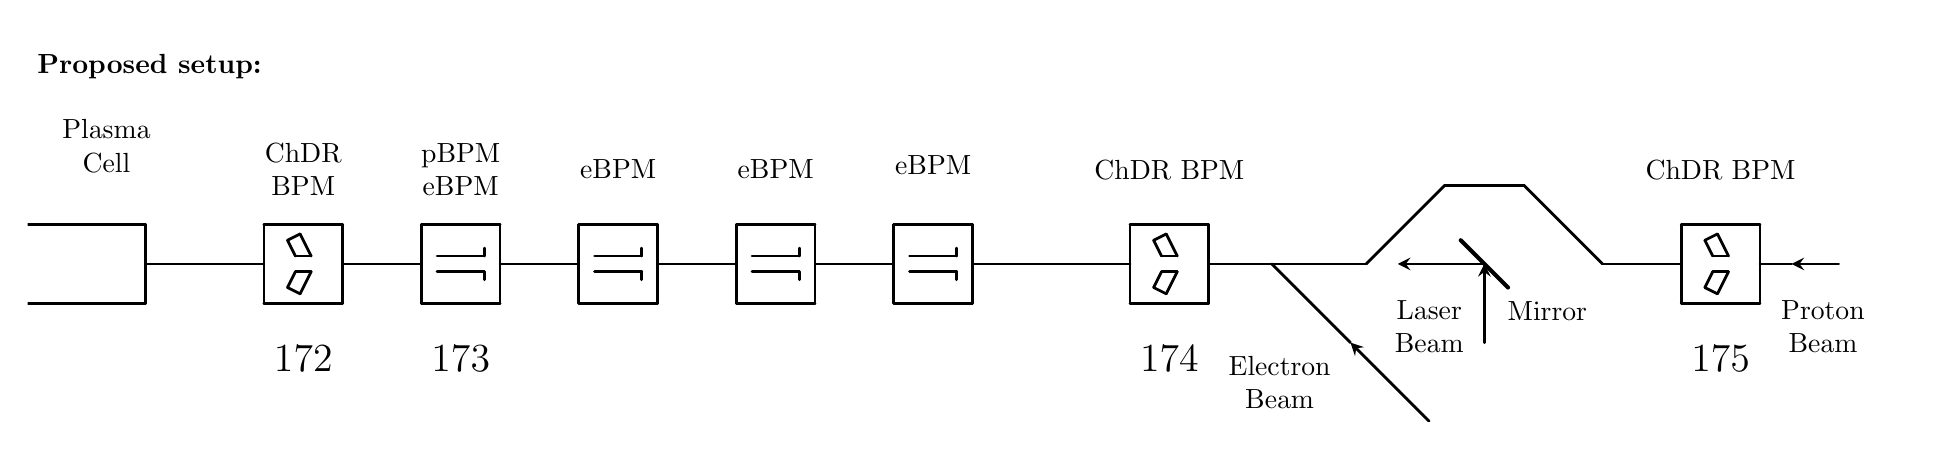
\begin{tikzpicture}[line cap=round,line join=round,>=stealth,x=1cm,y=1cm]
% new version
\clip(-10,-2) rectangle (14, 3);
\draw (-10.,2.5) node[anchor=west] {\textbf{Proposed setup:}};
\draw [line width=1pt] (-10,0.5)-- (-8.5,0.5);
\draw [line width=1pt] (-8.5,0.5)-- (-8.5,-0.5);
\draw [line width=1pt] (-8.5,-0.5)-- (-10,-0.5);
\draw (-9.,1.5) node[anchor=center] {\parbox{4cm}{\centering Plasma\\Cell}};
\draw [line width=1pt] (-7,0.5)-- (-7,-0.5);
\draw [line width=1pt] (-6,-0.5)-- (-6,0.5);
\draw [line width=1pt] (-6,0.5)-- (-7,0.5);
\draw [line width=1pt] (-7,-0.5)-- (-6,-0.5);
\draw [line width=1pt] (-5,0.5)-- (-5,-0.5);
\draw [line width=1pt] (-5,-0.5)-- (-4,-0.5);
\draw [line width=1pt] (-4,-0.5)-- (-4,0.5);
\draw [line width=1pt] (-4,0.5)-- (-5,0.5);
\draw [line width=1pt] (-3,0.5)-- (-3,-0.5);
\draw [line width=1pt] (-3,-0.5)-- (-2,-0.5);
\draw [line width=1pt] (-2,-0.5)-- (-2,0.5);
\draw [line width=1pt] (-2,0.5)-- (-3,0.5);
\draw [line width=1pt] (-1,0.5)-- (0,0.5);
\draw [line width=1pt] (0,0.5)-- (0,-0.5);
\draw [line width=1pt] (0,-0.5)-- (-1,-0.5);
\draw [line width=1pt] (-1,-0.5)-- (-1,0.5);
\draw [line width=1pt] (1,0.5)-- (1,-0.5);
\draw [line width=1pt] (1,-0.5)-- (2,-0.5);
\draw [line width=1pt] (2,-0.5)-- (2,0.5);
\draw [line width=1pt] (2,0.5)-- (1,0.5);
\draw [line width=1pt] (4,0.5)-- (5,0.5);
\draw [line width=1pt] (5,0.5)-- (5,-0.5);
\draw [line width=1pt] (5,-0.5)-- (4,-0.5);
\draw [line width=1pt] (4,-0.5)-- (4,0.5);
\draw [line width=1pt] (6,0)-- (5,0);
\draw [line width=1pt] (6,0)-- (7,0);
\draw [line width=1pt] (7,0)-- (8,1);
\draw [line width=1pt] (8,1)-- (9,1);
\draw [line width=1pt] (9,1)-- (10,0);
\draw [line width=1pt] (10,0)-- (11,0);
\draw [line width=1pt] (11,0.5)-- (12,0.5);
\draw [line width=1pt] (12,0.5)-- (12,-0.5);
\draw [line width=1pt] (12,-0.5)-- (11,-0.5);
\draw [line width=1pt] (11,0.5)-- (11,-0.5);
\draw [line width=1pt] (-8.5,0)-- (-7,0);
\draw [line width=1pt] (-6,0)-- (-5,0);
\draw [line width=1pt] (-4,0)-- (-3,0);
\draw [line width=1pt] (-2,0)-- (-1,0);
\draw [line width=1pt] (0,0)-- (1,0);
\draw [line width=1pt] (2,0)-- (4,0);
\draw [line width=1pt] (-4.8,0.1)-- (-4.2,0.1);
\draw [line width=1pt] (-4.2,0.1)-- (-4.2,0.2);
\draw [line width=1pt] (-4.8,-0.1)-- (-4.2,-0.1);
\draw [line width=1pt] (-4.2,-0.1)-- (-4.2,-0.2);
\draw [line width=1pt] (-2.8,0.1)-- (-2.2,0.1);
\draw [line width=1pt] (-2.2,0.1)-- (-2.2,0.2);
\draw [line width=1pt] (-2.8,-0.1)-- (-2.2,-0.1);
\draw [line width=1pt] (-2.2,-0.1)-- (-2.2,-0.2);
\draw [line width=1pt] (-0.8,0.1)-- (-0.2,0.1);
\draw [line width=1pt] (-0.2,0.1)-- (-0.2,0.2);
\draw [line width=1pt] (-0.8,-0.1)-- (-0.2,-0.1);
\draw [line width=1pt] (-0.2,-0.1)-- (-0.2,-0.2);
\draw [line width=1pt] (1.2,0.1)-- (1.8,0.1);
\draw [line width=1pt] (1.8,0.1)-- (1.8,0.2);
\draw [line width=1pt] (1.2,-0.1)-- (1.8,-0.1);
\draw [line width=1pt] (1.8,-0.1)-- (1.8,-0.2);
\draw [line width=1pt] (4.4,0.1)-- (4.6,0.1);
\draw [line width=1pt] (4.6,-0.1)-- (4.4,-0.1);
\draw [line width=1pt] (4.4,-0.1)-- (4.3,-0.3);
\draw [line width=1pt] (11.6,0.1)-- (11.4,0.1);
\draw [line width=1pt] (11.4,0.1)-- (11.3,0.3);
\draw [line width=1pt] (11.6,-0.1)-- (11.4,-0.1);
\draw [line width=1pt] (11.4,-0.1)-- (11.3,-0.3);
\draw [line width=1pt] (11.46,0.38)-- (11.6,0.1);
\draw [line width=1pt] (11.46,0.38)-- (11.3,0.3);
\draw [line width=1pt] (11.3,-0.3)-- (11.46,-0.38);
\draw [line width=1pt] (11.6,-0.1)-- (11.46,-0.38);
\draw [line width=1pt] (4.3,0.3)-- (4.46,0.38);
\draw [line width=1pt] (4.46,0.38)-- (4.6,0.1);
\draw [line width=1pt] (4.3,-0.3)-- (4.46,-0.38);
\draw [line width=1pt] (4.46,-0.38)-- (4.6,-0.1);
\draw [line width=1pt] (-6.6,0.1)-- (-6.4,0.1);
\draw [line width=1pt] (-6.6,0.1)-- (-6.7,0.3);
\draw [line width=1pt] (-6.4,0.1)-- (-6.54,0.38);
\draw [line width=1pt] (-6.7,0.3)-- (-6.54,0.38);
\draw [line width=1pt] (-6.6,-0.1)-- (-6.4,-0.1);
\draw [line width=1pt] (-6.6,-0.1)-- (-6.7,-0.3);
\draw [line width=1pt] (-6.4,-0.1)-- (-6.54,-0.38);
\draw [line width=1pt] (-6.7,-0.3)-- (-6.54,-0.38);

\draw (-6.5,1.2) node[anchor=center]  {\parbox{4cm}{\centering ChDR\\BPM}};
\draw (-4.5,1.2) node[anchor=center] {\parbox{4cm}{\centering pBPM\\eBPM}};
\draw (-2.5,1.2) node[anchor=center] {eBPM};
\draw (-0.5,1.2) node[anchor=center] {eBPM};
\draw (1.5,1.25) node[anchor=center] {eBPM};
\draw [line width=1pt] (4.3,0.3)-- (4.4,0.1);
\draw (4.5,1.2) node[anchor=center] {ChDR BPM};
\draw (11.5,1.2) node[anchor=center] {ChDR BPM};
\draw [line width=1.5pt] (8.2,0.3)-- (8.8,-0.3);
\draw [->,line width=1pt] (8.5,-1) -- (8.5,0);
\draw [->,line width=1pt] (8.5,0) -- (7.4,0);
\draw (7.8,-0.8) node[anchor=center]  {\parbox{4cm}{\centering Laser\\Beam}};;
\draw (9.3,-0.6) node[anchor=center] {Mirror};
\draw [->,line width=1pt] (13,0) -- (12.4,0);
\draw [line width=1pt] (12.4,0)-- (12,0);
\draw (12.8,-0.8) node[anchor=center]  {\parbox{4cm}{\centering Proton\\Beam}};;
\draw [line width=1pt] (5.8,0)-- (6.8,-1);
\draw [->,line width=1pt] (7.8,-2) -- (6.8,-1);
\draw (5.9,-1.5) node[anchor=center]  {\parbox{4cm}{\centering Electron\\Beam}};;

\draw (-6.5,-1.2) node[anchor=center]  {\Large\ding{172}};
\draw (-4.5,-1.2) node[anchor=center]  {\Large\ding{173}};
\draw (4.5,-1.2) node[anchor=center]  {\Large\ding{174}};
\draw (11.5,-1.2) node[anchor=center]  {\Large\ding{175}};

\end{tikzpicture}

\caption{Layout of the present AWAKE BPM systems and the proposed modifications. The proton BPMs (pBPM) are electrostatic buttons, the electron BPMs (eBPM) are shorted striplines. The proposed modifications are: \ding{172}: convert the pBPM into a ChDR BPM, \ding{173}: use the eBPM to measure also the proton position by splitting its signal, \ding{174}: install a new ChDR BPM in a drift space, \ding{175}: install a ChDR BPM in the proton beamline to measure the proton beam power in the ChDR BPM detection band.}
\label{fig:awake_layout_fd}
\end{figure}
\end{landscape}














